\documentclass[12pt]{article}
\rmfamily
\usepackage[margin=1.0in]{geometry}
\usepackage{graphicx}
\graphicspath{ {figures/} }

\title{TCP Dynamics Report}
\date{November 2020}
\author{Will Goodman}

\begin{document}
\maketitle

All data for this report was gathered using a Python script with the "requests" library and a 60 second timeout.

\section{Analysing the strategy of the client and server to maintain throughput on ports 4030 through 4039}
\subsection*{Investigation}
The data for this part was collected between 8PM and 11PM on the evening of Sunday 1st November.
My strategy was to use Wireshark to capture downloads of different size files on the same port.
I then investigated what happened when the throughput was zero and how the client and server worked together to get the throughput flowing again.

\subsubsection*{Low loss, small file (Port 4032, 256KB):}
To begin investigating the strategy of the client and server, I analysed how a 256KB file was downloaded from port 4032 (10\% packet loss).
Initial inspection revealed the following:
\begin{itemize}
  \item The client's buffer is 64240 bytes
  \item Each TCP packet payload received from the server is 1452 bytes
  \item The sequence number of the packet is the cumulative number of payload bytes, including the current packet
  \item The cumulative acknowledgements from the client to the server refer to the next expected packet (as per TCP specification)
  \item The client sends an ACK after every two packets have been received
\end{itemize}

By reviewing a graph of the throughput, we can see "plateaux" where no data is being transferred (figure \ref{figure1: 4032:256KB Throughput}).

\begin{figure}[!htbp]
  \centering
  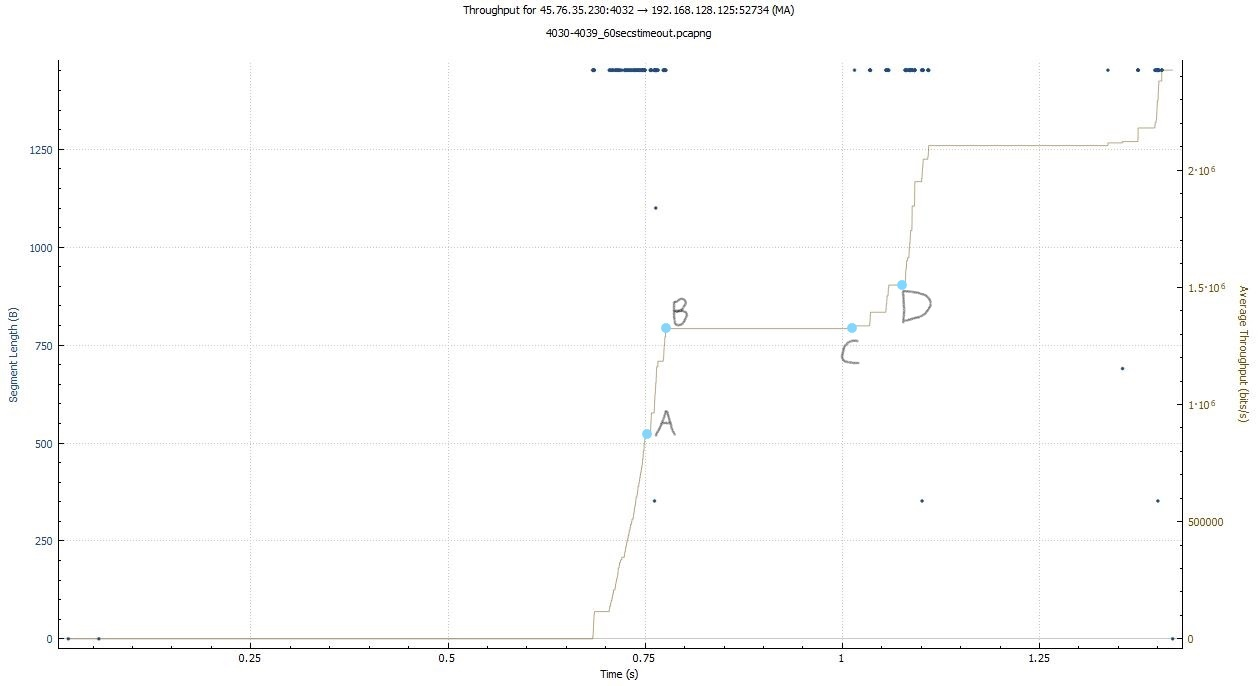
\includegraphics[scale=0.3]{4032_256KB_throughput-marked-points.jpg}
  \caption{"256KB file, port 4032 (10\%) packet loss throughput."}
  \label{figure1: 4032:256KB Throughput}
\end{figure}

Upon reviewing the packet capture, we can see that the throughput has a slight reduction when the first duplicate ACK is sent (packet 217034 in figure \ref{figure2: first duplicate ACK} is point A in figure \ref{figure1: 4032:256KB Throughput}).
Following the first duplicate ACK, it appears the server continues to send packets for 250 milliseconds before resending the missing packet, despite the client returning duplicate ACKs stating a packet has not arrived.

\begin{figure}[!htbp]
  \centering
  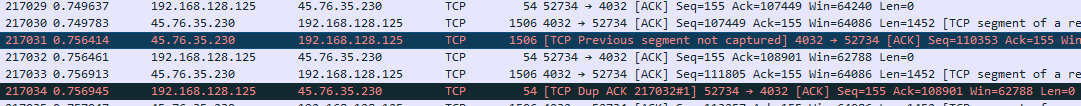
\includegraphics[width=\linewidth]{4032-256KB-duplicate-ack.PNG}
  \caption{"First duplicate ACK."}
  \label{figure2: first duplicate ACK}
\end{figure}

In total, thirty-nine duplicate ACKs are sent before the packet is retransmitted by the server.
Normally, we would expect a Fast Retransmission to be triggered after three duplicate ACKs are received.
Instead, a regular Retransmission occurs, which is usually triggered by a timeout rather than a duplicate ACK.
Either the duplicate ACKs are not arriving at the server, or it does not use Fast Retransmission in the standard way.
Fast Retransmission does occur as expected later in the TCP stream (described in more detail later in the report), so it must be the former.

\begin{figure}[!htbp]
  \centering
  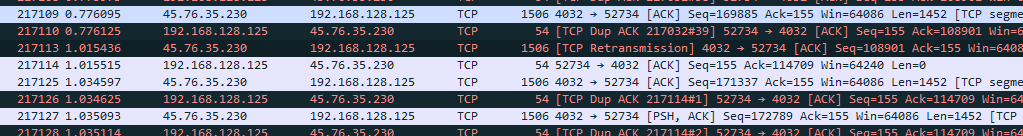
\includegraphics[width=\linewidth]{4032-256KB-retransmission.PNG}
  \caption{"First retransmission."}
  \label{figure4: First retransmission}
\end{figure}

As we know this Retransmission is triggered by the server timing out waiting for an ACK, we can estimate the length of the timeout.
We look at the time taken between the client sending the oldest ACK for the first time, and when the retransmission is received to make this estimate.
In figure \ref{figure2: first duplicate ACK} line 217032 (ACK) is at 0.756461 seconds and in figure \ref{figure4: First retransmission} line 217113 (retransmission) is at 1.015436 seconds.
This is a time difference of 0.258975.
Later in the TCP trace another packet goes missing, and the time difference is 0.250174.
From these two values we can estimate that the timeout for the oldest unacknowledged packet on the server is a quarter of a second.

Another interesting feature we can see here is TCP flow control.
The 250 milliseconds of packets the server sends after the first duplicate ACK do not overflow the client's buffer.
By looking at figure \ref{figure3: BIF and Window Size}, we can see that the number of bytes-in-flight never exceeds the Window Size.
The peak of the BIF (where the buffer would overflow), is the point where the server retransmits the missing packet.
From this we can assume that the server limits the number of unacknowledged packets which have been sent to not exceed the client's buffer space (TCP Flow Control).

\begin{figure}[!htbp]
  \centering
  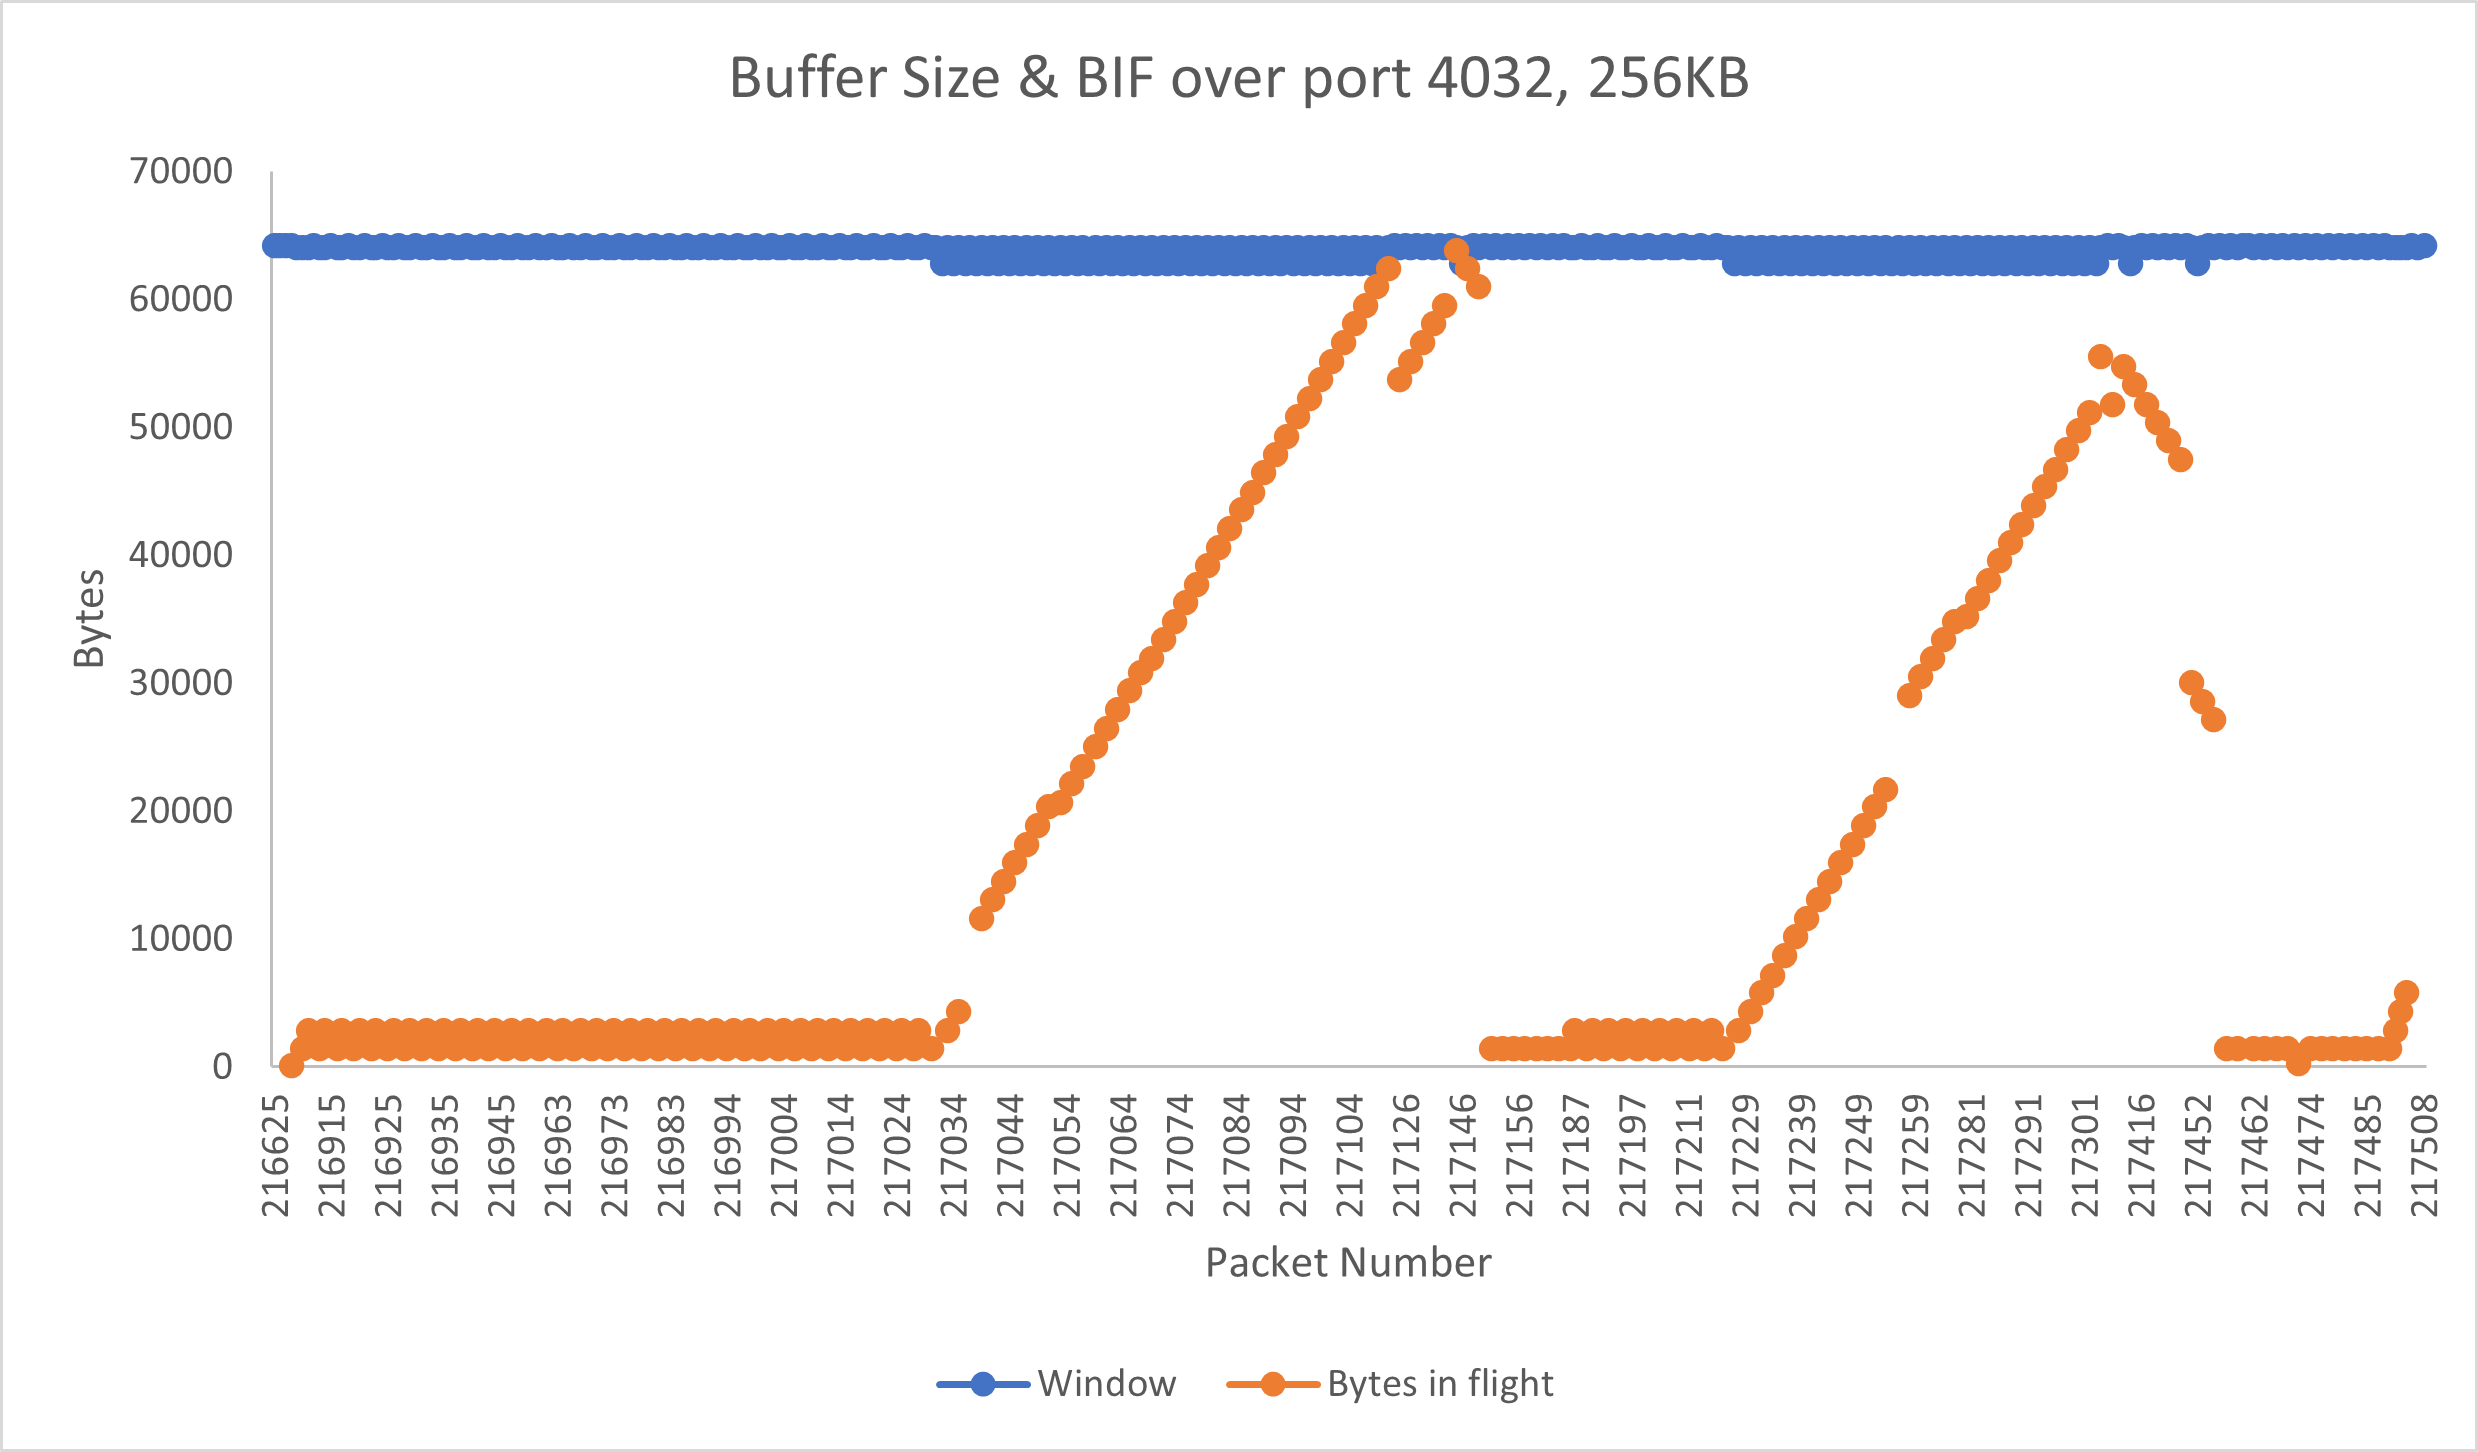
\includegraphics[width=\linewidth]{4032-256KB-bytes-in-flight.png}
  \caption{"Bytes-in-Flight in comparison to Window Size."}
  \label{figure3: BIF and Window Size}
\end{figure}

Once it has resent the missing packet, the server continues where it left off and continues sending packets it has not already sent.
This is seen in figure \ref{figure4: First retransmission}, where the server transmits sequence 169885, then retransmits sequence 108901.
Retransmission of 108901 is point C in figure \ref{figure1: 4032:256KB Throughput}
The first packet the server sends after the retransmission is 171337, which is the next in the sequence (169885 + 1452 bytes = 171337).
This shows that the server is aware the client is buffering all out-of-order packets, and is not discarding them like a pipelined receiver.

In this case something interesting happens.
It appears a second packet had actually gone missing (114709), and so the client sends another duplicate ACK.
As the client receives more out-of-order packets, four more duplicate ACKs are sent.
On the server, this appears to trigger a Rapid Recovery/Fast Retransmission as the server starts retransmitting every packet after 114709 (see figure \ref{figure5: Fast retransmission}).

\begin{figure}[!htbp]
  \centering
  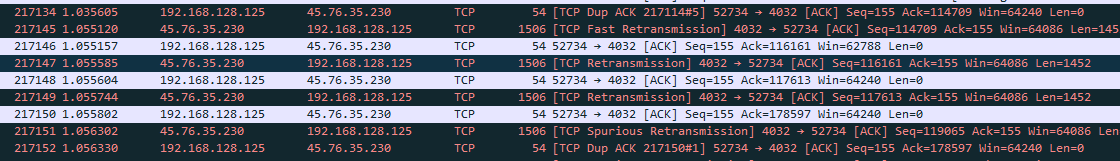
\includegraphics[width=\linewidth]{4032-256KB-fast-retransmission.PNG}
  \caption{"Fast retransmission."}
  \label{figure5: Fast retransmission}
\end{figure}

As a cumulative acknowledgement is being used, the server only knows that every packet up to sequence 114709 has been received, it does not know the status of every packet it has sent since.
As three duplicate ACKs have been received for the same missing packet, a Fast Retransmission is triggered and every packet since the missing packet is retransmitted.
In this case, only four packets went missing (sequence 108901, 114709, 116161, 117613), and so every packet after this has already been received and buffered (causing a spurious retransmission).
When the spurious transmissions start occuring, the client responds with duplicate ACKs stating that all these packets are being retransmitted unnecessarily.
Eventually, the server receives one of these duplicate ACKs, and starts sending packets as normal (figure \ref{figure6: Return to normal}, and point D on \ref{figure1: 4032:256KB Throughput}).

\begin{figure}[!htbp]
  \centering
  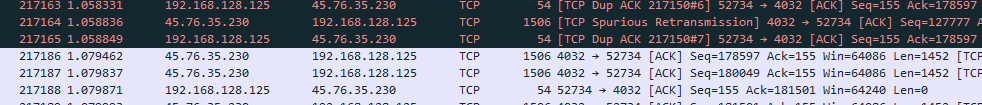
\includegraphics[width=\linewidth]{4032-256KB-back-to-normal.PNG}
  \caption{"Return to normal."}
  \label{figure6: Return to normal}
\end{figure}

The question arises, why did the first missing packet not cause a Fast Retransmission but the second did?
As mentioned earlier, this is likely because some or all of the duplicate ACKs did not reach the server.
This may also be the reason five duplicate ACKs were sent before the Fast Retransmission of the second missing packet was triggered, as opposed to the three duplicate ACKs required by the specification. 

Further evidence of ACKs going missing appears lower within the TCP stream (figure \ref{figure7: Missing ACKs}).
A collection of packets are retransmitted despite acknowledgements being sent by the client (spurious retransmissions).
The duplicate ACKs for packet sequence 232321 must arrive however, as the Fast Retransmission is triggered for that packet.

\begin{figure}[!htbp]
  \centering
  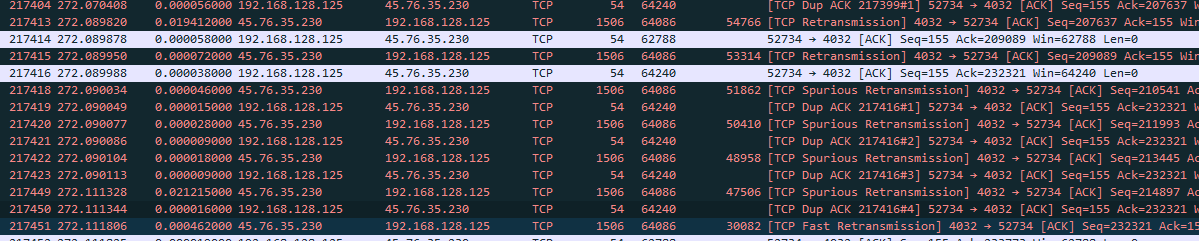
\includegraphics[width=\linewidth]{4032-256KB-lost-acks.PNG}
  \caption{"ACKs going missing."}
  \label{figure7: Missing ACKs}
\end{figure}

Another feature which is worth noting, is the server does not appear to be using Slow Start.
This is unexpected, as Slow Start should be compulsory.
In figure \ref{figure3: BIF and Window Size} we can see that the number of bytes-in-flight stays stable at 2904, unless a packet has been unacknowledged.
If Slow Start was in use, we would expect to see this increase exponentially until a packet has been lost.

\subsubsection*{Low loss, medium file (Port 4032, 16MB):}
With a larger file, we begin to see how both the client and server deal with packet loss over a longer period of time.

By looking at the packet capture, we can see that the same behaviour of acknowledgements and retransmissions occurs for the larger file as it did for the smaller file.
This 16Mb file never actually finished downloading, the client ended the connection before it completed (figure \ref{figure8: 4032:16M RST}).

\begin{figure}[!htbp]
  \centering
  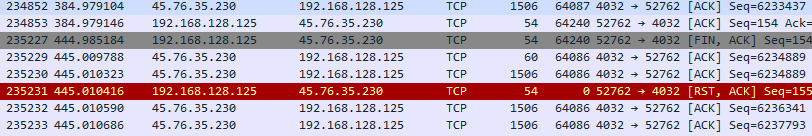
\includegraphics[width=\linewidth]{4032-16M-RST.PNG}
  \caption{"Client RST."}
  \label{figure8: 4032:16M RST}
\end{figure}

Upon further inspection we can see the last contact from the server (234852) is at 384.979104 seconds.
60 seconds later (235227), the client sends a FIN, ACK packet to close the connection.
This is triggered by the timeout within the Python script used to collect the data (mentioned at start of report).
After this FIN, ACK packet, the client receives a regular packet from the server. 
This packet was likely already in the wire when the FIN, ACK was received by the server.
Due to this, the client sends a RST, ACK packet to terminate the connection completely.

\subsection*{Client/Server Strategy}
\subsubsection*{Client}
Following the investigation, I believe this is the Client's strategy to attempt to maintain throughput:
\begin{itemize}
  \item Send a cumulative ACK after receiving every two packets
  \item If an out-of-order packet is received, an ACK is sent stating what the next expected packet is
  \item If another out-of-order packet is received, a duplicate ACK is sent. This repeats until the missing packet is received
  \item All out-of-order packets are buffered
  \item If a duplicate packet is received, then a duplicate ACK is sent
  \item When the last packet arrives, send a FIN, ACK to close the connection
  \item If no packets from the server for 60 seconds, send a FIN, ACK to close the connection
  \item If any packets are received from the server after sending a FIN, ACK (excluding an acknowledgement of the FIN, ACK), send a RST, ACK packet
\end{itemize}

I was not able to investigate whether Silly Window Syndrome would occur as the client appeared to move packets from the buffer to the application very quickly, and as such found no occurrences where the Window Size was zero.
In order to try and trigger this I tried downloading large files (32MB, 64MB) with both Python and with wget within the Windows terminal, with no luck.

\subsubsection*{Server}
The server knows less about which packets have been received correctly than the client, so it has a slightly more complicated strategy.
\begin{itemize}
  \item Send packets in order, pipelining packets without waiting for acknowledgement
  \item Use a congestion window of 2 packets
  \item If a packet has not been acknowledged after quarter of a second, just resend that packet. Assume all packets sent since that packet have arrived correctly and pick up where you left off after it is resent
  \item If you receive three duplicate ACKs for a packet, assume all packets from that sequence number on have been lost and resend them all (Rapid Recovery)
  \item If you receive a duplicate ACK from the client stating that more packets have arrived than previously thought, stop resending packets before that sequence number and start sending subsequent packets
  \item If you receive a FIN, ACK from the client, assume all packets have been received correctly (or the client wants to stop the connection for another reason)
\end{itemize}

\section{Analysing Drop In Performance As Packets Are Lost}
The data for this part was collected between 8PM and 11PM on the evening of Sunday 1st November.

To begin, let's look at how long it takes to download the same file on different ports.
Figure \ref{figure9: 4030-4039:16KB download time}, shows the median time (out of five attempts) to download a 16KB file on ports 4030 to 4039. 

\begin{figure}[!htbp]
  \centering
  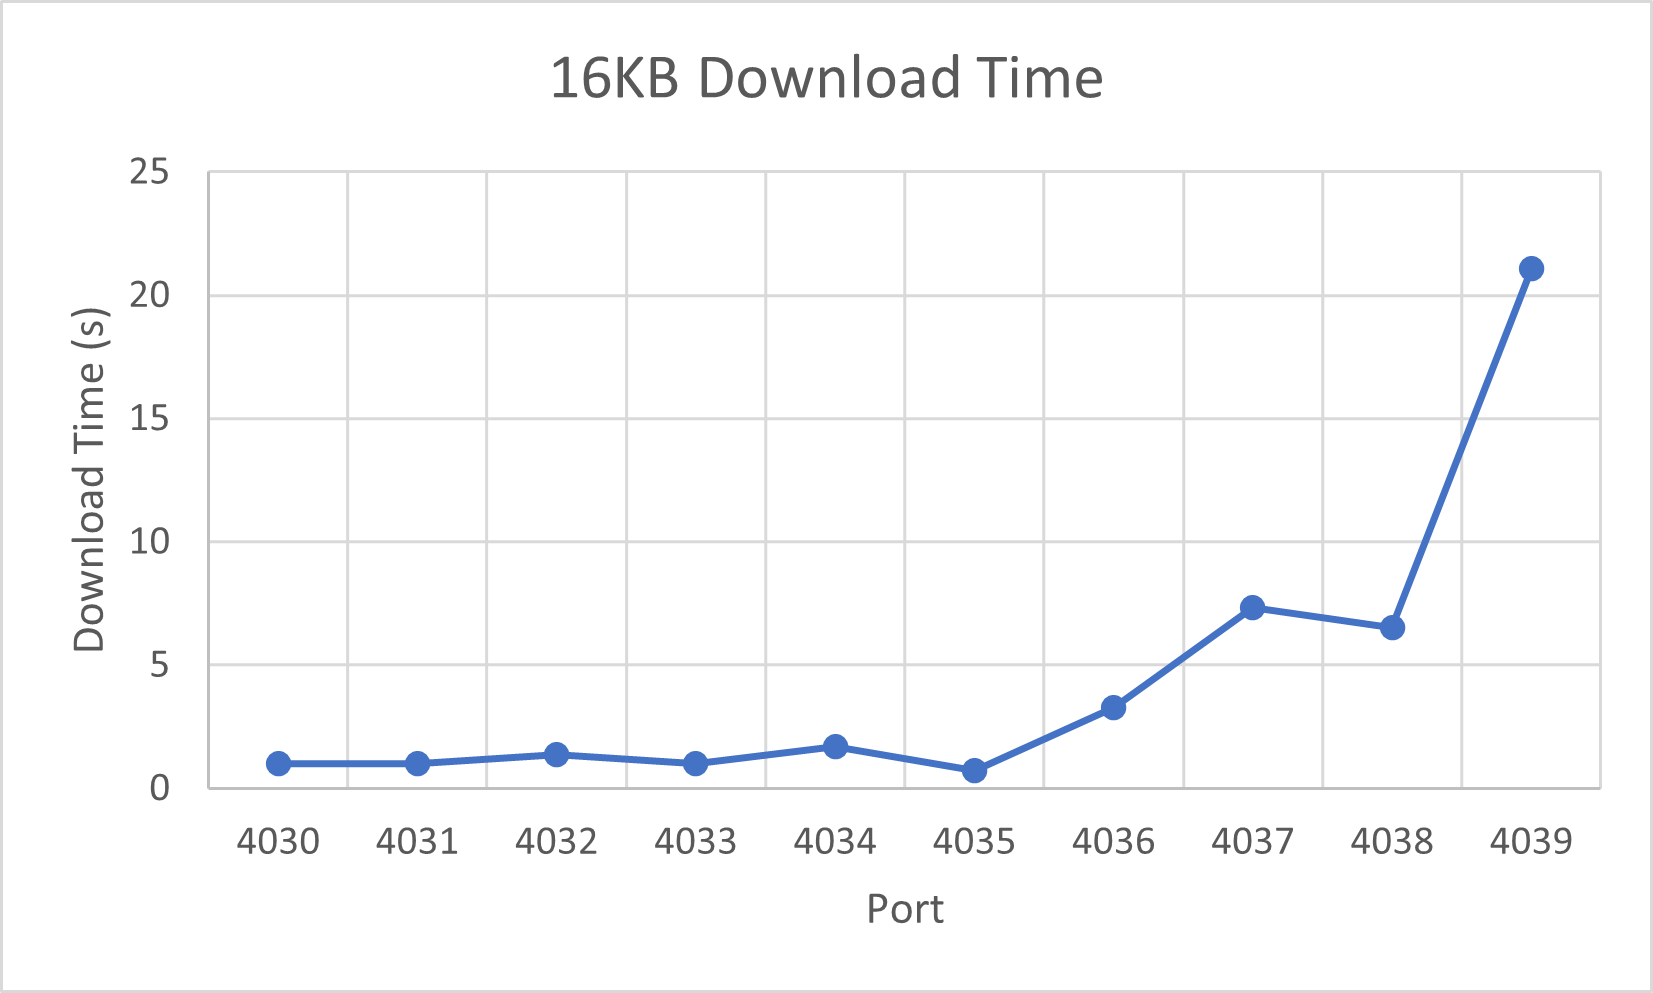
\includegraphics[width=\linewidth]{4030-4039-16KB-download-time.png}
  \caption{"4030-4039:16KB download time."}
  \label{figure9: 4030-4039:16KB download time}
\end{figure}

In the lower ports, up until port 4036, there is very little change in download time.
From port 4036 onwards, we start to see an exponential increase in download time.
If we look at 64KB, we see a similar picture and some of the more lossy ports (4037 onwards) start to timeout (figure \ref{figure10: 4030-4039:64KB download time}).
The only difference here is that the curve starts to become exponential earlier, at 15\% packet loss rather than 30\%.

\begin{figure}[!htbp]
  \centering
  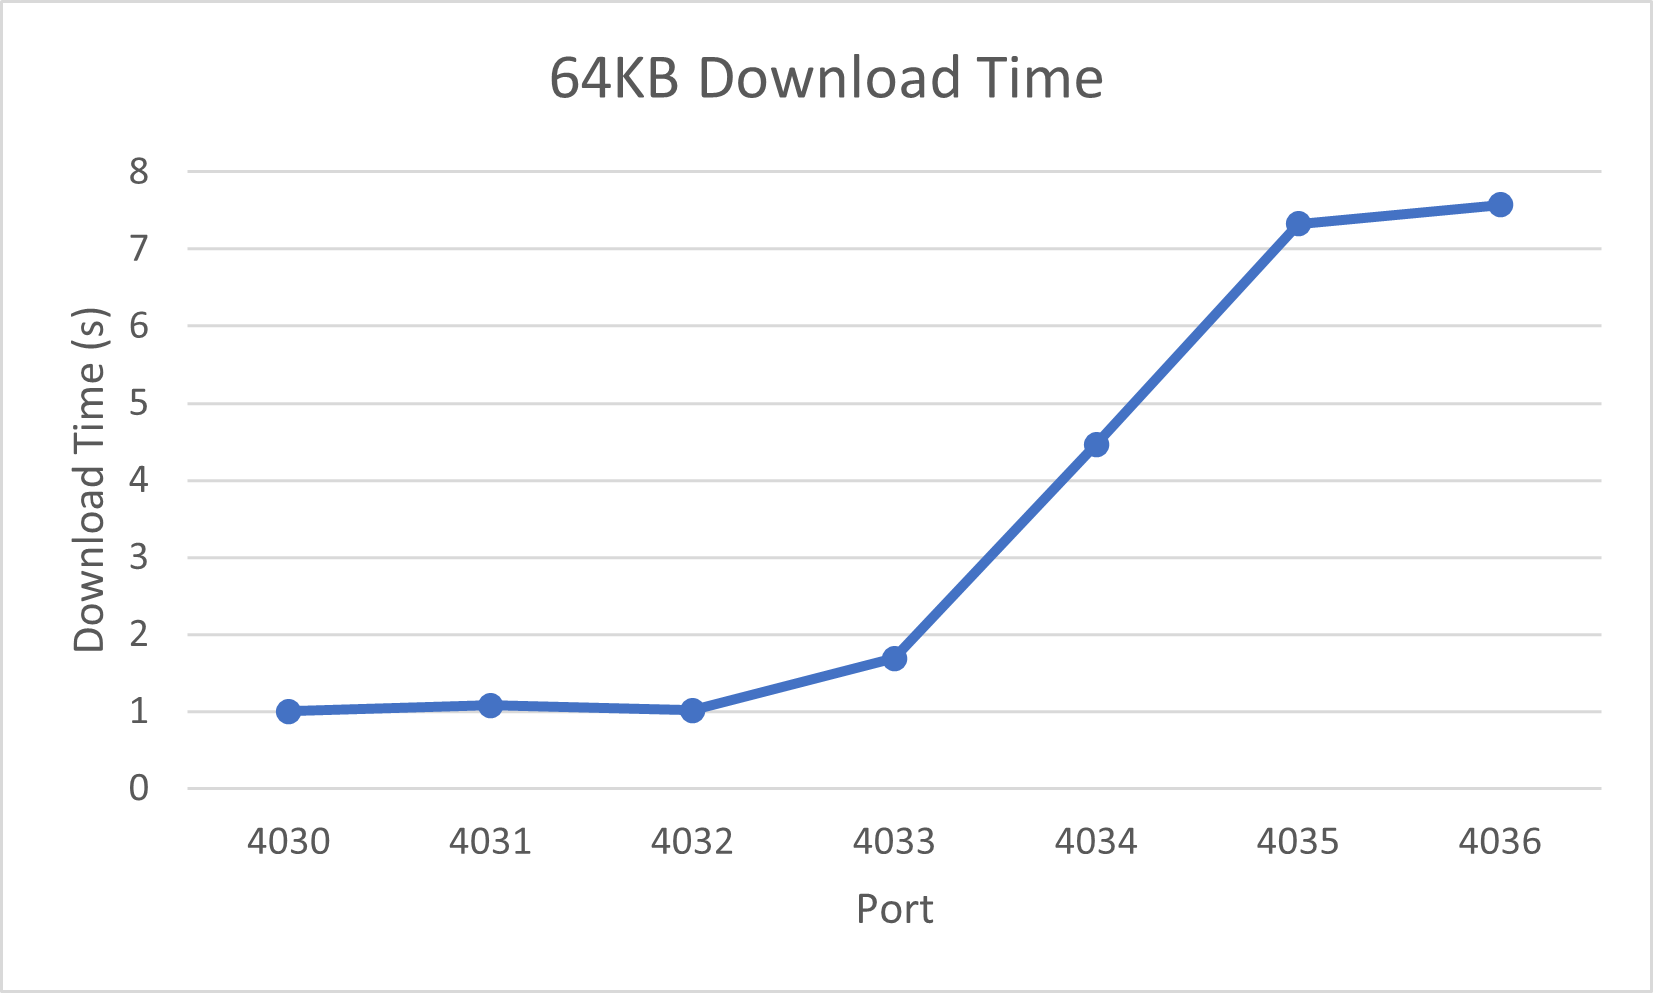
\includegraphics[width=\linewidth]{4030-4039-64KB-download.png}
  \caption{"4030-4039:64KB download time."}
  \label{figure10: 4030-4039:64KB download time}
\end{figure}

The same pattern is seen with a 2MB file (figure \ref{figure11: 4030-4039:2MB download time}).
Download time appears to increase exponentially as packet loss increases.
In addition, packet loss appears to affect the performance of downloading larger files much more than smaller files.

\begin{figure}[!htbp]
  \centering
  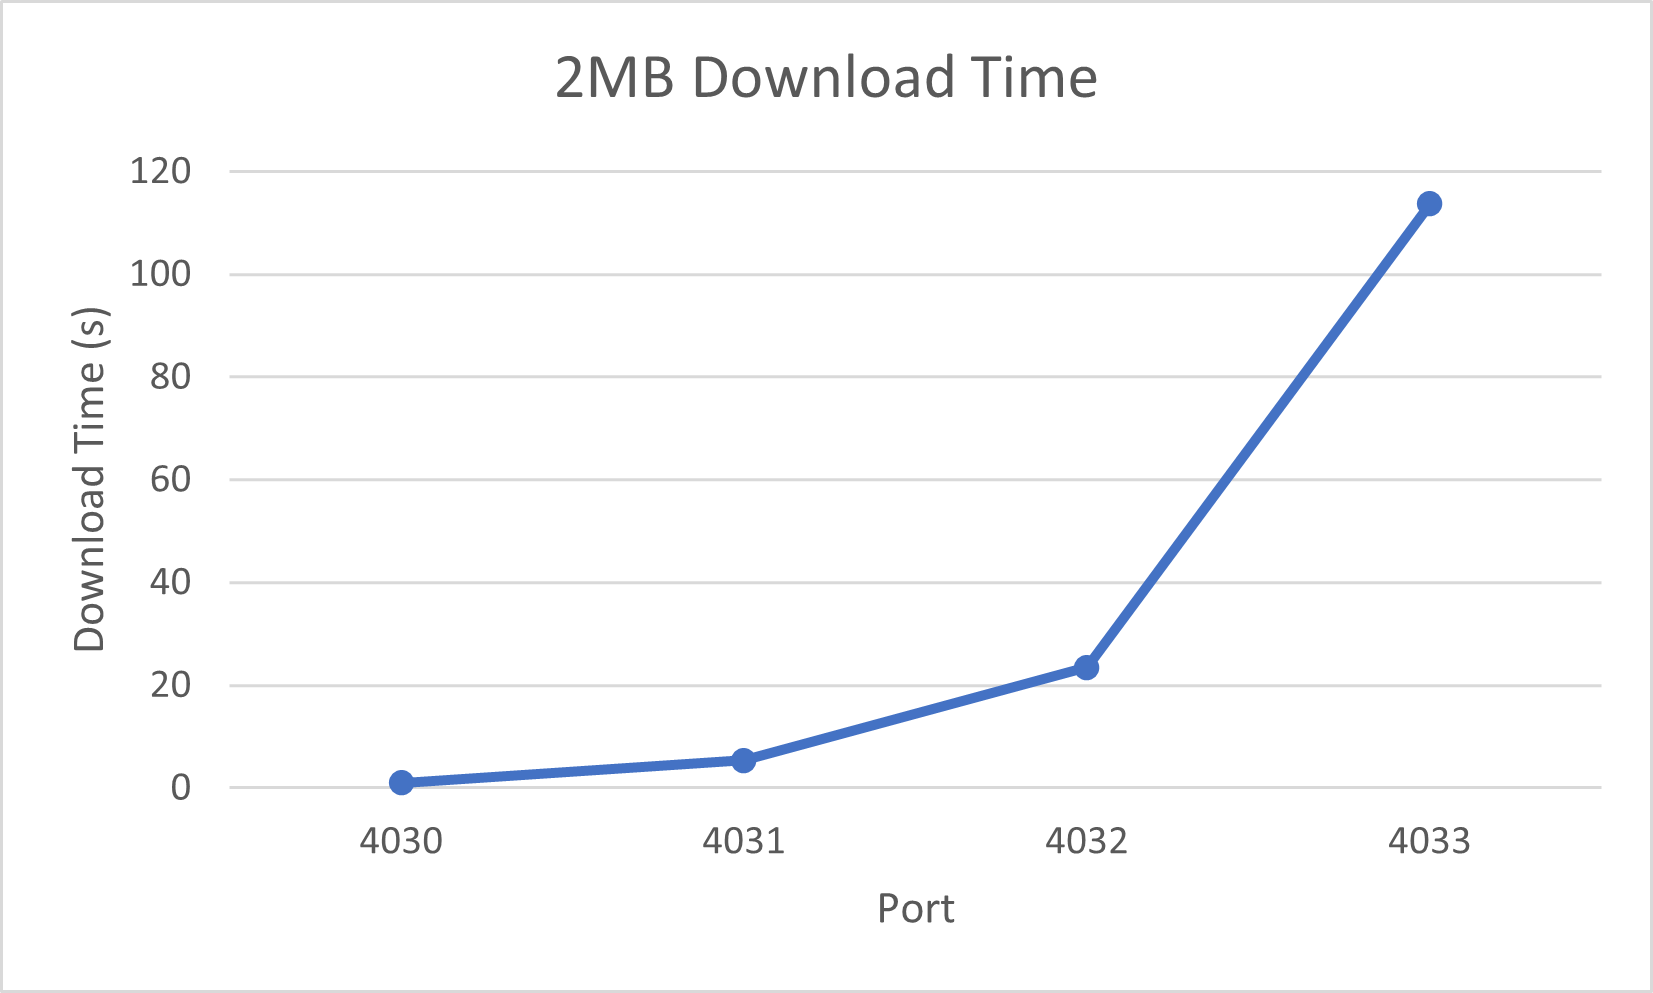
\includegraphics[width=\linewidth]{4030-4039-2MB-download-time.png}
  \caption{"4030-4039:2MB download time."}
  \label{figure11: 4030-4039:2MB download time}
\end{figure}

Why is this?
If we look at figure \ref{figure12: 4035:256KB tcptrace}, we can see increasingly long periods where no packets are received from the server.
At a first glance, these periods appear to double in length each time, an exponential backoff.

\begin{figure}[!htbp]
  \centering
  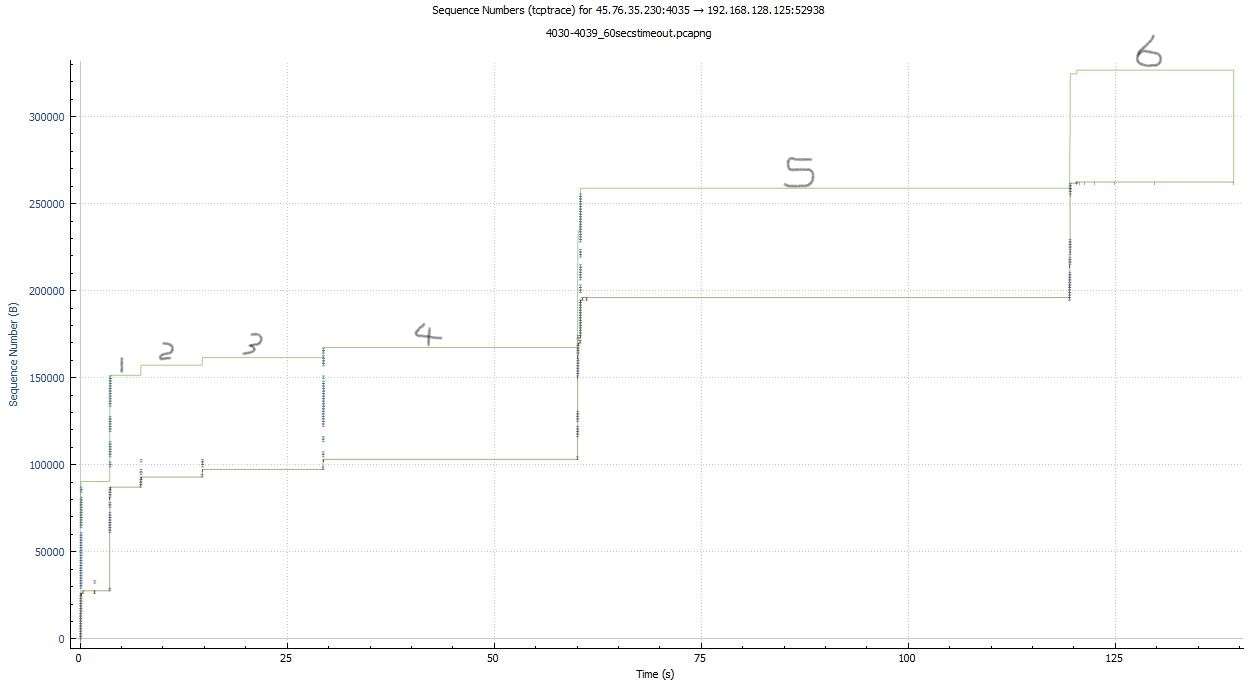
\includegraphics[width=\linewidth]{4035-256KB-tcptrace.jpg}
  \caption{"4035:256KB (25\% loss) tcptrace."}
  \label{figure12: 4035:256KB tcptrace}
\end{figure}

By looking at the timings of the packets within the TCP stream, we can see this to be true:
\begin{enumerate}
  \item 1987.344151 - 1983.34451 = 3.99964 seconds
  \item 1994.448845 - 1987.076671 = 7.37217 seconds
  \item 2009.034187 - 1994.478403 = 14.55578 seconds
  \item 2039.757708 - 2009.098606 = 30.6591 seconds
  \item 2099.158037 - 2040.852611 = 58.30542 seconds
\end{enumerate}

The pauses are not exactly double each other, however this would be expected as packets may take slightly less or more time to reach the client from the server.
The values are close enough for us to assume our hypothesis is correct, and there is an exponential backoff on the server.
This is why the client ends the connection before pause six ends, as pause six would be 120 seconds, and the client has a 60 second timeout.
This backoff is the reason we see an exponential trend as packet loss increases.
The curve increases more aggressively for larger files as there are more packets which can go missing.

This exponential backoff is known as Karn's Algorithm.
Each time the timer expires and triggers a retransmission, the server increases the timeout by multiplying the current timeout by a value.
According to the algorithm, the value does not need to be two, however it typically is and in this case clearly is.
Generally, the intial timeout is an estimate of the round-trip time plus some safety margin, and in this case is likely 3 and a half seconds.

\section{Analysing performance with and without Selective Acknowledgement and Window Scaling}
The data for this part was collected on 5th November.

To compare performance between the different configurations, we need to see how they perform downloading the same file with different percentages of packet loss.
I downloaded a 16KB file from each port (4000-4039) five times, and plotted the median on figure \ref{figure13: 4000-4039:16KB Average Download Time}.
By using the median rather than the mean, I removed the anomalous results.

By looking at the graph, we can see that there is very little difference between the configurations with low amounts of loss.
Once the percentage of lost packets breaks 30\% (ports 40X6), the different configurations start to become separated.
Having both Selective Acknowledgement and Window Scaling enabled results in the best performance, with a very minimal increase in download time as packet loss increases.
Window Scaling and Selective Acknowledgement enabled independently provide very similar results, however Window Scaling does appear to provide slightly better performance.
Both Window Scaling and Selective Acknowledgement disabled provides by far the worst performance, however the result for port 4039 is so much worse than 4009, 4019, and 4029, that I would not be surprised if there were other network issues at play.

\begin{figure}[!htbp]
  \centering
  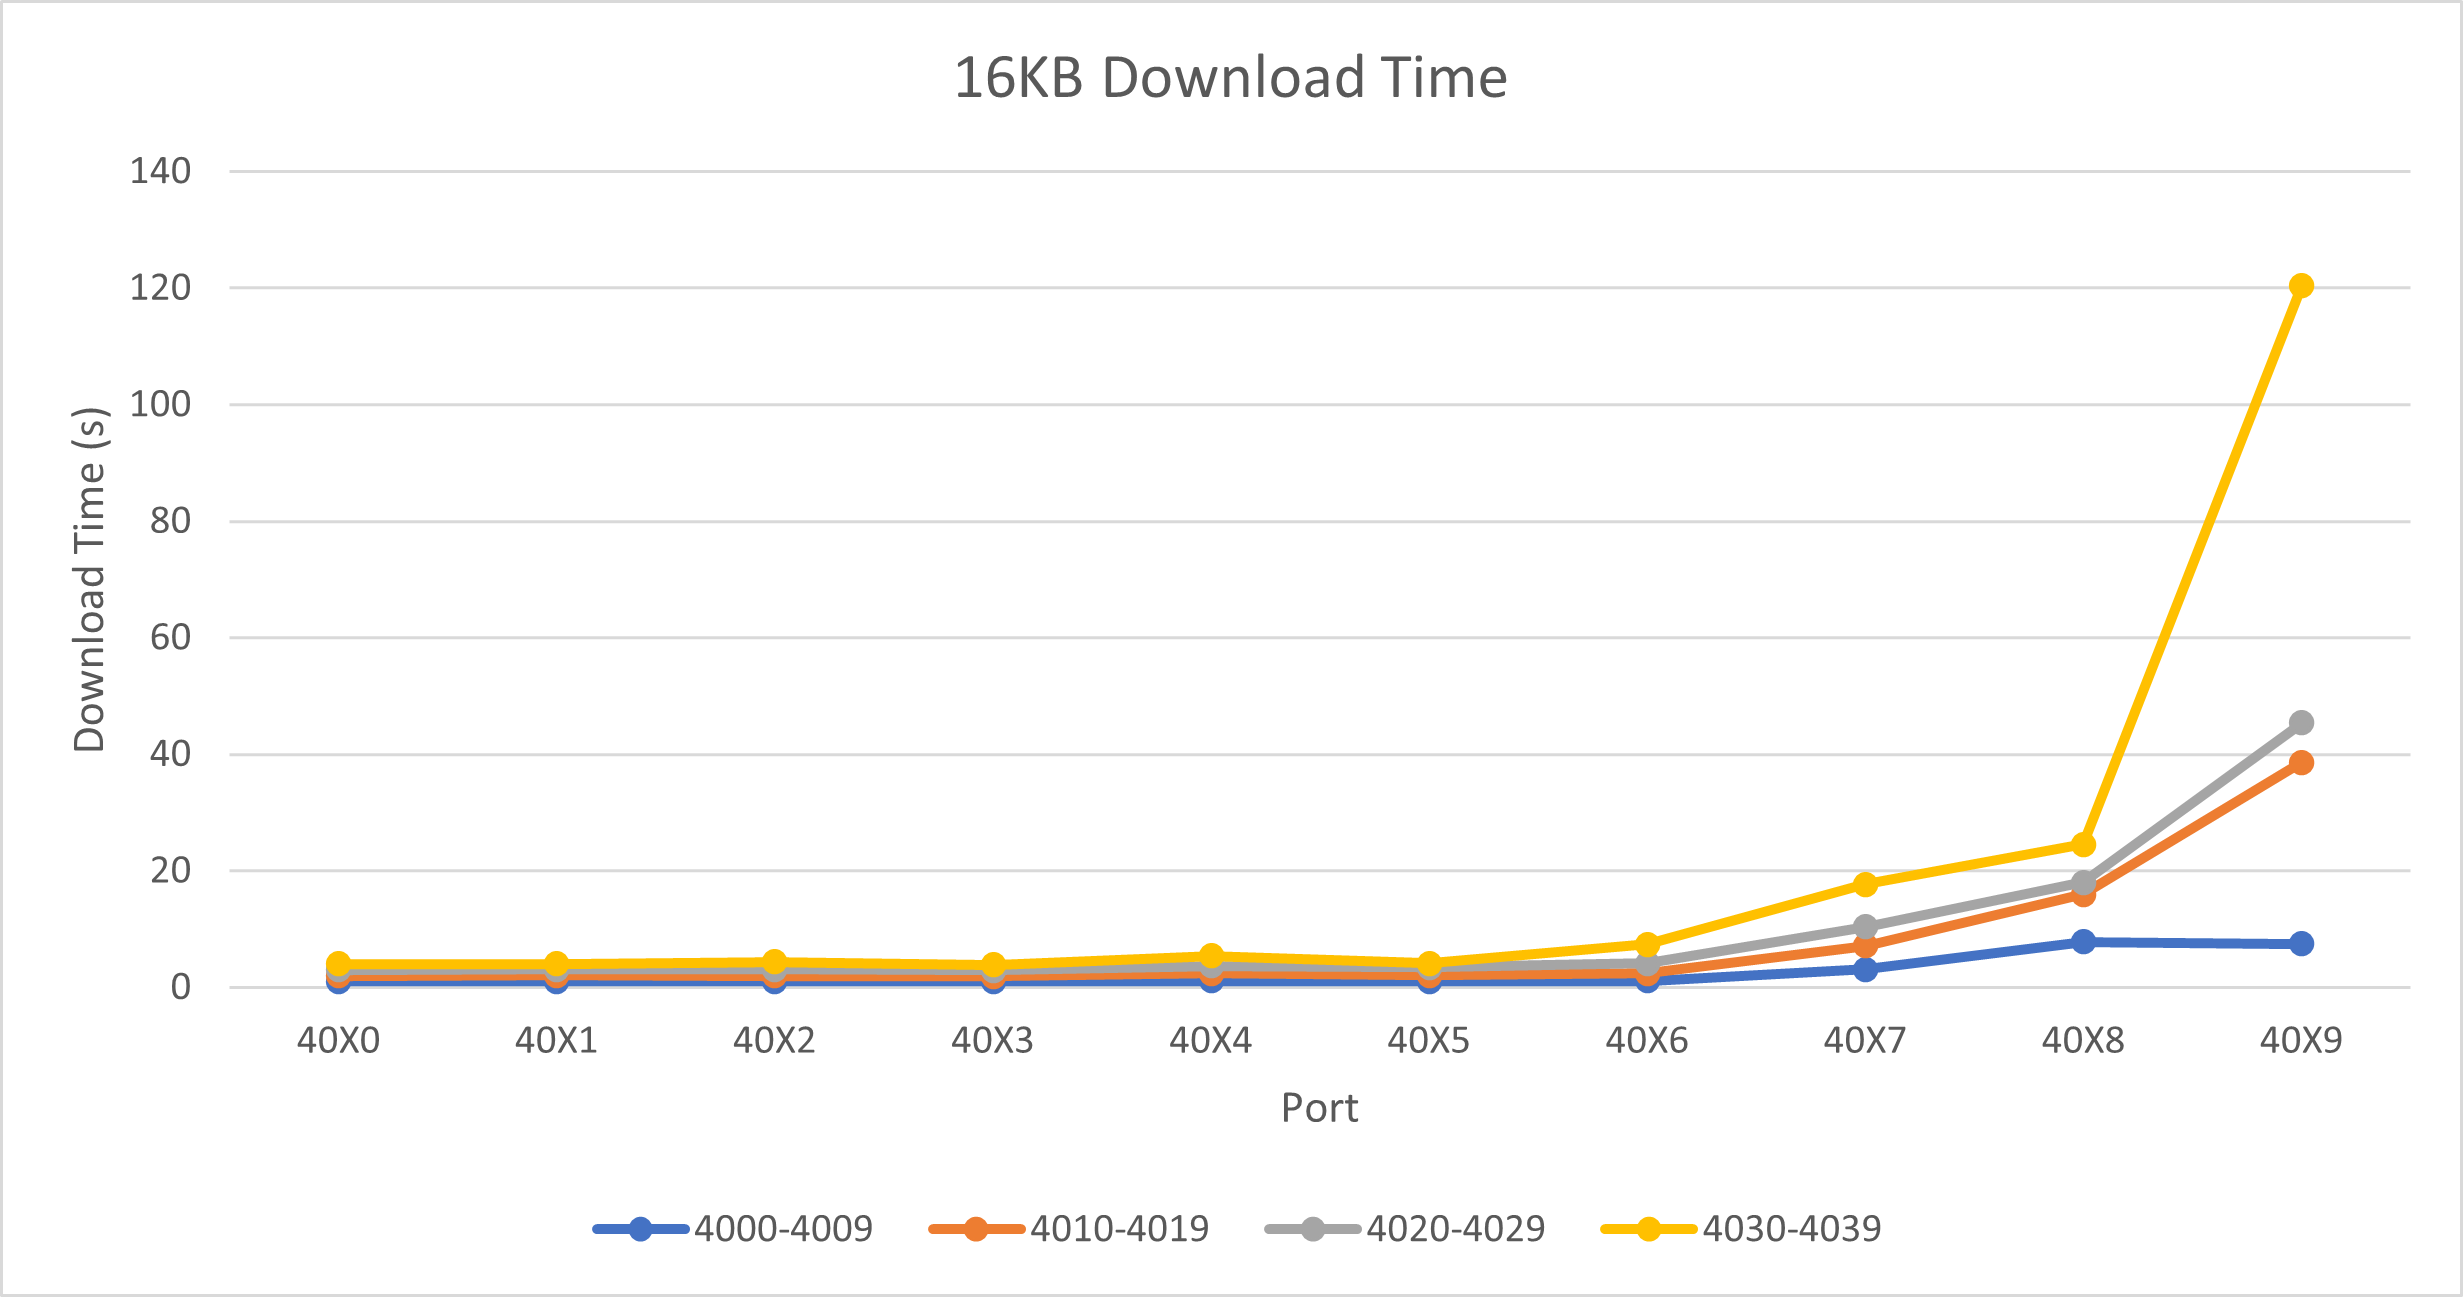
\includegraphics[width=\linewidth]{4000-4039-16KB-download-time.png}
  \caption{"4000-4039:16KB Average Download Time."}
  \label{figure13: 4000-4039:16KB Average Download Time}
\end{figure}

However, 16KB is not a very large file, and as such there are not that many packets which are able to be lost.
If we perform the same experiment on a larger file, 2MB, we may be able to confirm our assumptions.

\begin{figure}[!htbp]
  \centering
  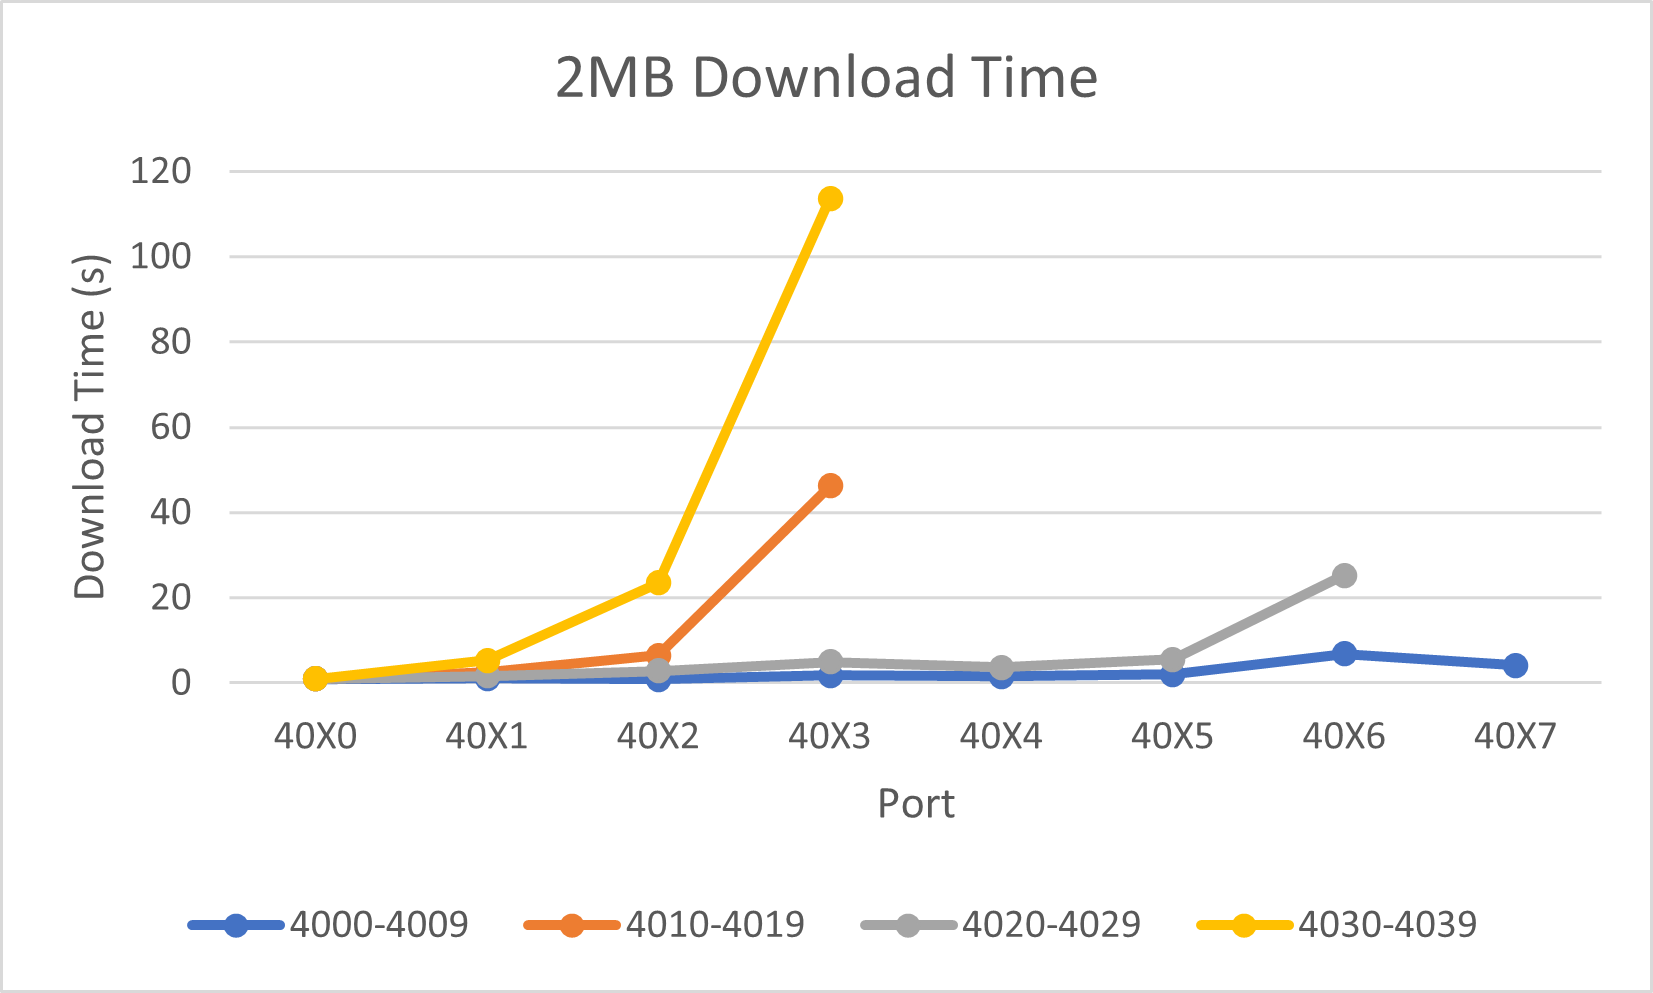
\includegraphics[width=\linewidth]{4000-4039-2MB-download-time.png}
  \caption{"4000-4039:2MB Average Download Time."}
  \label{figure14: 4000-4039:2MB Average Download Time}
\end{figure}

In figure \ref{figure14: 4000-4039:2MB Average Download Time}, we see that the results for Selective Acknowledgement and Window Scaling either all enabled or all disabled are vaguely the same as before.
However, the results for just having Selective Acknowledgement enabled seem to outperform results for just Window Scaling.
Since ports 4010 and 4020 are very similar, and when downloading a small file Window Scaling and Selective Acknowledgement perform very similarly, could Selective Acknowledgement just be dealing better with packet loss?

If we look at an even larger file of 16MB (figure \ref{figure15: 4000-4039:16MB Average Download Time}), it becomes clear.

\begin{figure}[!htbp]
  \centering
  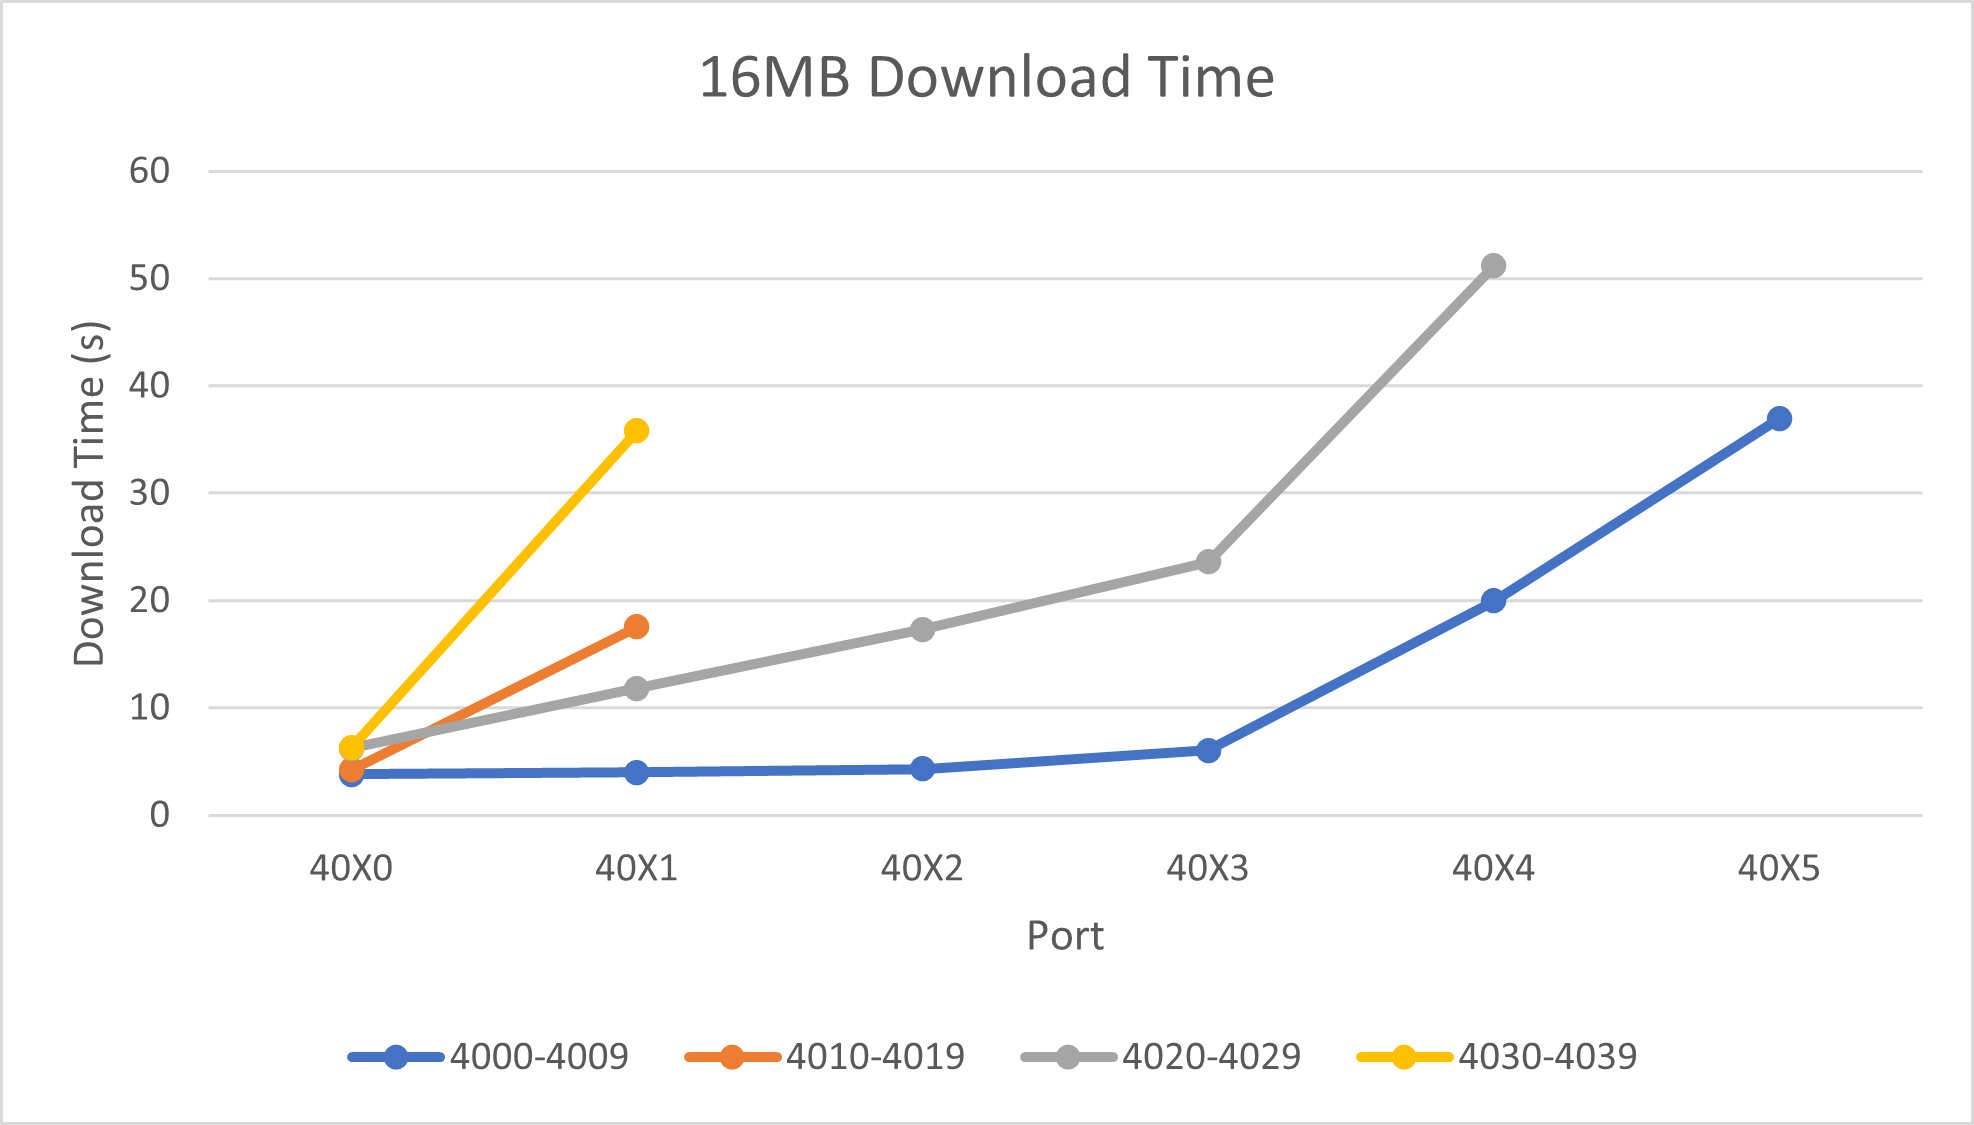
\includegraphics[width=\linewidth]{4000-4039-16MB-download-time.png}
  \caption{"4000-4039:16MB Average Download Time."}
  \label{figure15: 4000-4039:16MB Average Download Time}
\end{figure}

With just Window Scaling enabled, the download timed out with only 10\% packet loss.
With just Selective Acknowledgement enabled, the download did not time out until 35\% packet loss, and the performance is much improved over Window Scaling.

Selective Acknowledgement does not outperform Window Scaling in all scenarios, however.
In the case of 0\% packet loss, such as in figure \ref{figure16: 64MB Average Download Time}, Window Scaling significantly outperforms Selective Acknowledgement.
This makes sense, as Window Scaling allows more data to be sent quicker, and if no (or very few) packets are lost then the data will be delivered quicker.
It also makes sense that Selective Acknowledgement will give better performance when there is packet loss, as it will allow the client and server to recover quicker.
With SA, the server knows exactly which packets have arrived, and will only resend those which have definitely not arrived.
Without SA, the server will have to resend many packets which have potentially already been delivered successfully, taking up space within the Window which could have been used for new packets, and prolonging the time taken to deliver all packets. 

\begin{figure}[!htbp]
  \centering
  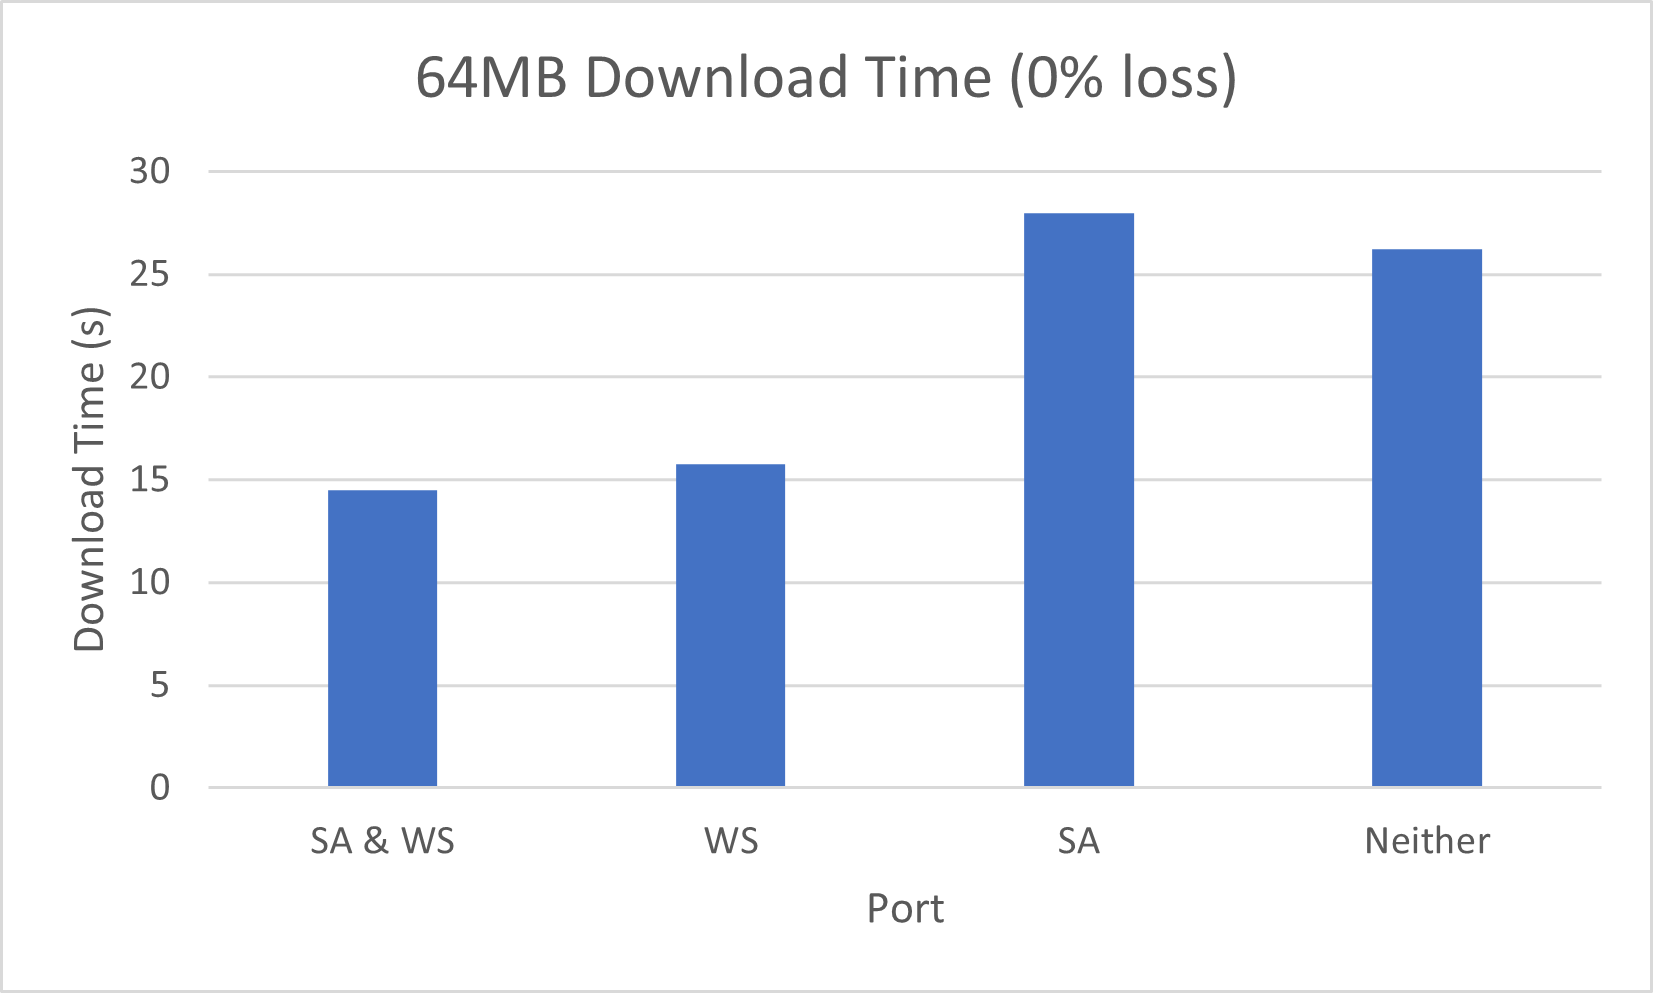
\includegraphics[width=\linewidth]{64MB-no-loss-download-time.png}
  \caption{"64MB Average Download Time."}
  \label{figure16: 64MB Average Download Time}
\end{figure}

In conclusion, the best results are always achieved with Selective Acknowledgement and Window Scaling enabled, and the worst results occur when both are disabled.
In reliable networks, Window Scaling will make a larger improvement, and in lossy networks, Selective Acknowledgement is more important.

\end{document}